\documentclass[11pt, twoside]{article}
\usepackage{boisik}
\usepackage[OT1]{fontenc}
\usepackage[affil-it]{authblk}
\usepackage{graphicx}
\usepackage{textcomp}
\usepackage{multicol}
\usepackage{natbib}
\usepackage{geometry}
\usepackage{amsmath}
\usepackage{lineno}
\usepackage[dvipsnames]{xcolor}
\usepackage{hyperref}
\hypersetup{
    colorlinks,
    linkcolor={red!50!black},
    citecolor={blue!50!black},
    urlcolor={blue!80!black}
}
\usepackage{xcolor}
\usepackage{float}
\usepackage{wrapfig}
<<<<<<< Updated upstream
\usepackage[belowskip=-10pt,aboveskip=0pt]{caption}
=======
\usepackage{caption}
>>>>>>> Stashed changes
\captionsetup[figure]{font=small,labelfont=normalsize}


\linenumbers
 \geometry{a4paper, total={170mm,257mm}, left=20mm, top=20mm}

\renewcommand{\baselinestretch}{1.3}

\title{\huge Perceptual Similarities Among Wallpaper Group Exemplars}
\author[1,2]{Peter J. Kohler}
\author[3]{Shivam Vedak}
\author[3]{Rick O. Gilmore}

\affil[1]{\small York University, Department of Psychology, Toronto, ON M3J 1P3, Canada}
\affil[2]{\small Centre for Vision Research, York University, Toronto, ON, M3J 1P3, Canada}
\affil[3]{\small Department of Psychology, Penn State University, Pennsylvania, USA}

\date{}

\begin{document}

\maketitle

% about 200 words
\begin{abstract}Symmetries are abundant within the visual environment, and many animals species are sensitive to visual symmetries. Wallpaper groups a class of 17 regular textures that each contain a distinct combination of the four fundamental symmetries, translation, reflection, rotation and glide reflection, and together represent the complete set of possible symmetries in two-dimensional images. Wallpapers are visually compelling and elicit responses in visual brain areas that precisely capture the symmetry content of each group, in humans and other primates. Here we ask to what extent exemplars from the same wallpaper group are perceptually similar. We algorithmically produce a set of well-matched exemplars from 5 of the 17 wallpaper groups and instructed participants to freely sort the exemplars from each group into as many subsets as they wished based on any criteria they saw appropriate. \textit{P1}, the simplest of the 17 groups, was consistently rated more self-similar than any other group, while the other four groups, although varying in symmetry content, were comparable in self-similarity. Our results suggest that except for the most extreme case (\textit{P1}), self-similarity of wallpaper groups is not directly tied to symmetry content.\end{abstract}

\section*{Introduction}
Symmetry has been recognized as important for human visual perception since the late 19th century \citep{mach_1959}. In the two spatial dimensions relevant for images, symmetries can be combined in 17 distinct ways, \textit{the wallpaper groups} \citep{RN1562,RN1563,RN1425}. Wallpaper groups are different from the stimuli typically used to probe the role of symmetry in visual perception in two ways: First, they contain combinations of the four fundamental symmetry types translation, reflection, rotation and glide reflection, rather than just reflection or mirror symmetry, which has been the focus of most vision research. Second, the symmetries in wallpaper groups are repeated to tile the plane, rather than positioned at a single image location as is usually the case. These differences, and the fact that wallpaper groups together form the complete set of symmetries possible in the two-dimensional image plane, make wallpapers an interesting stimulus set for studying perception of visual symmetries.
<<<<<<< Updated upstream
\begin{wrapfigure}{r}{0.4\textwidth}
	\centering
	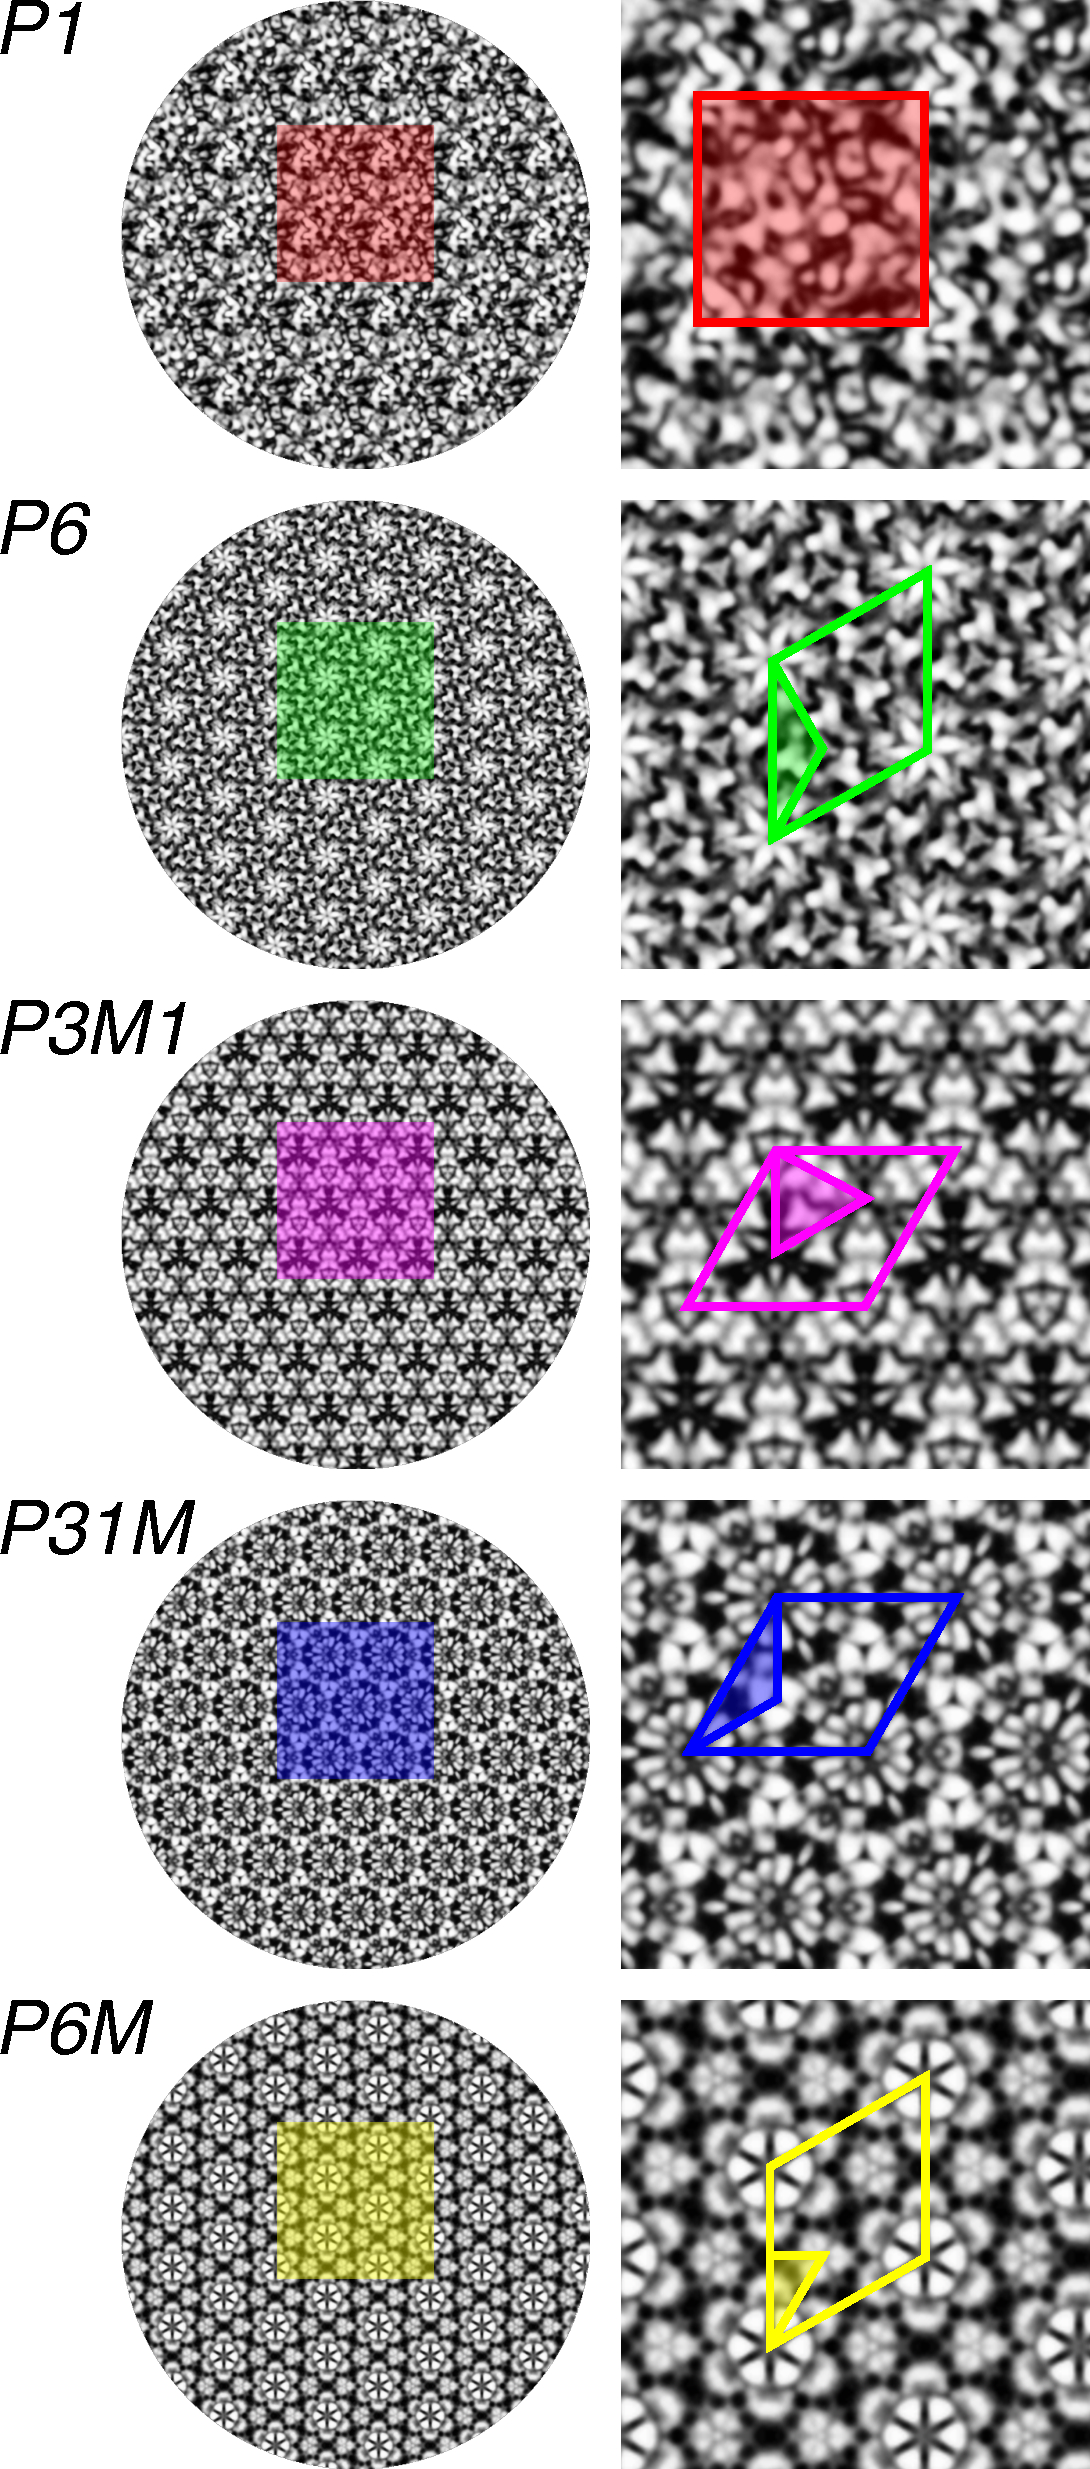
\includegraphics[width=0.38\textwidth]{./figures/wpg_structure.pdf}
=======
\begin{wrapfigure}{r}{0.46\textwidth}
	\centering
	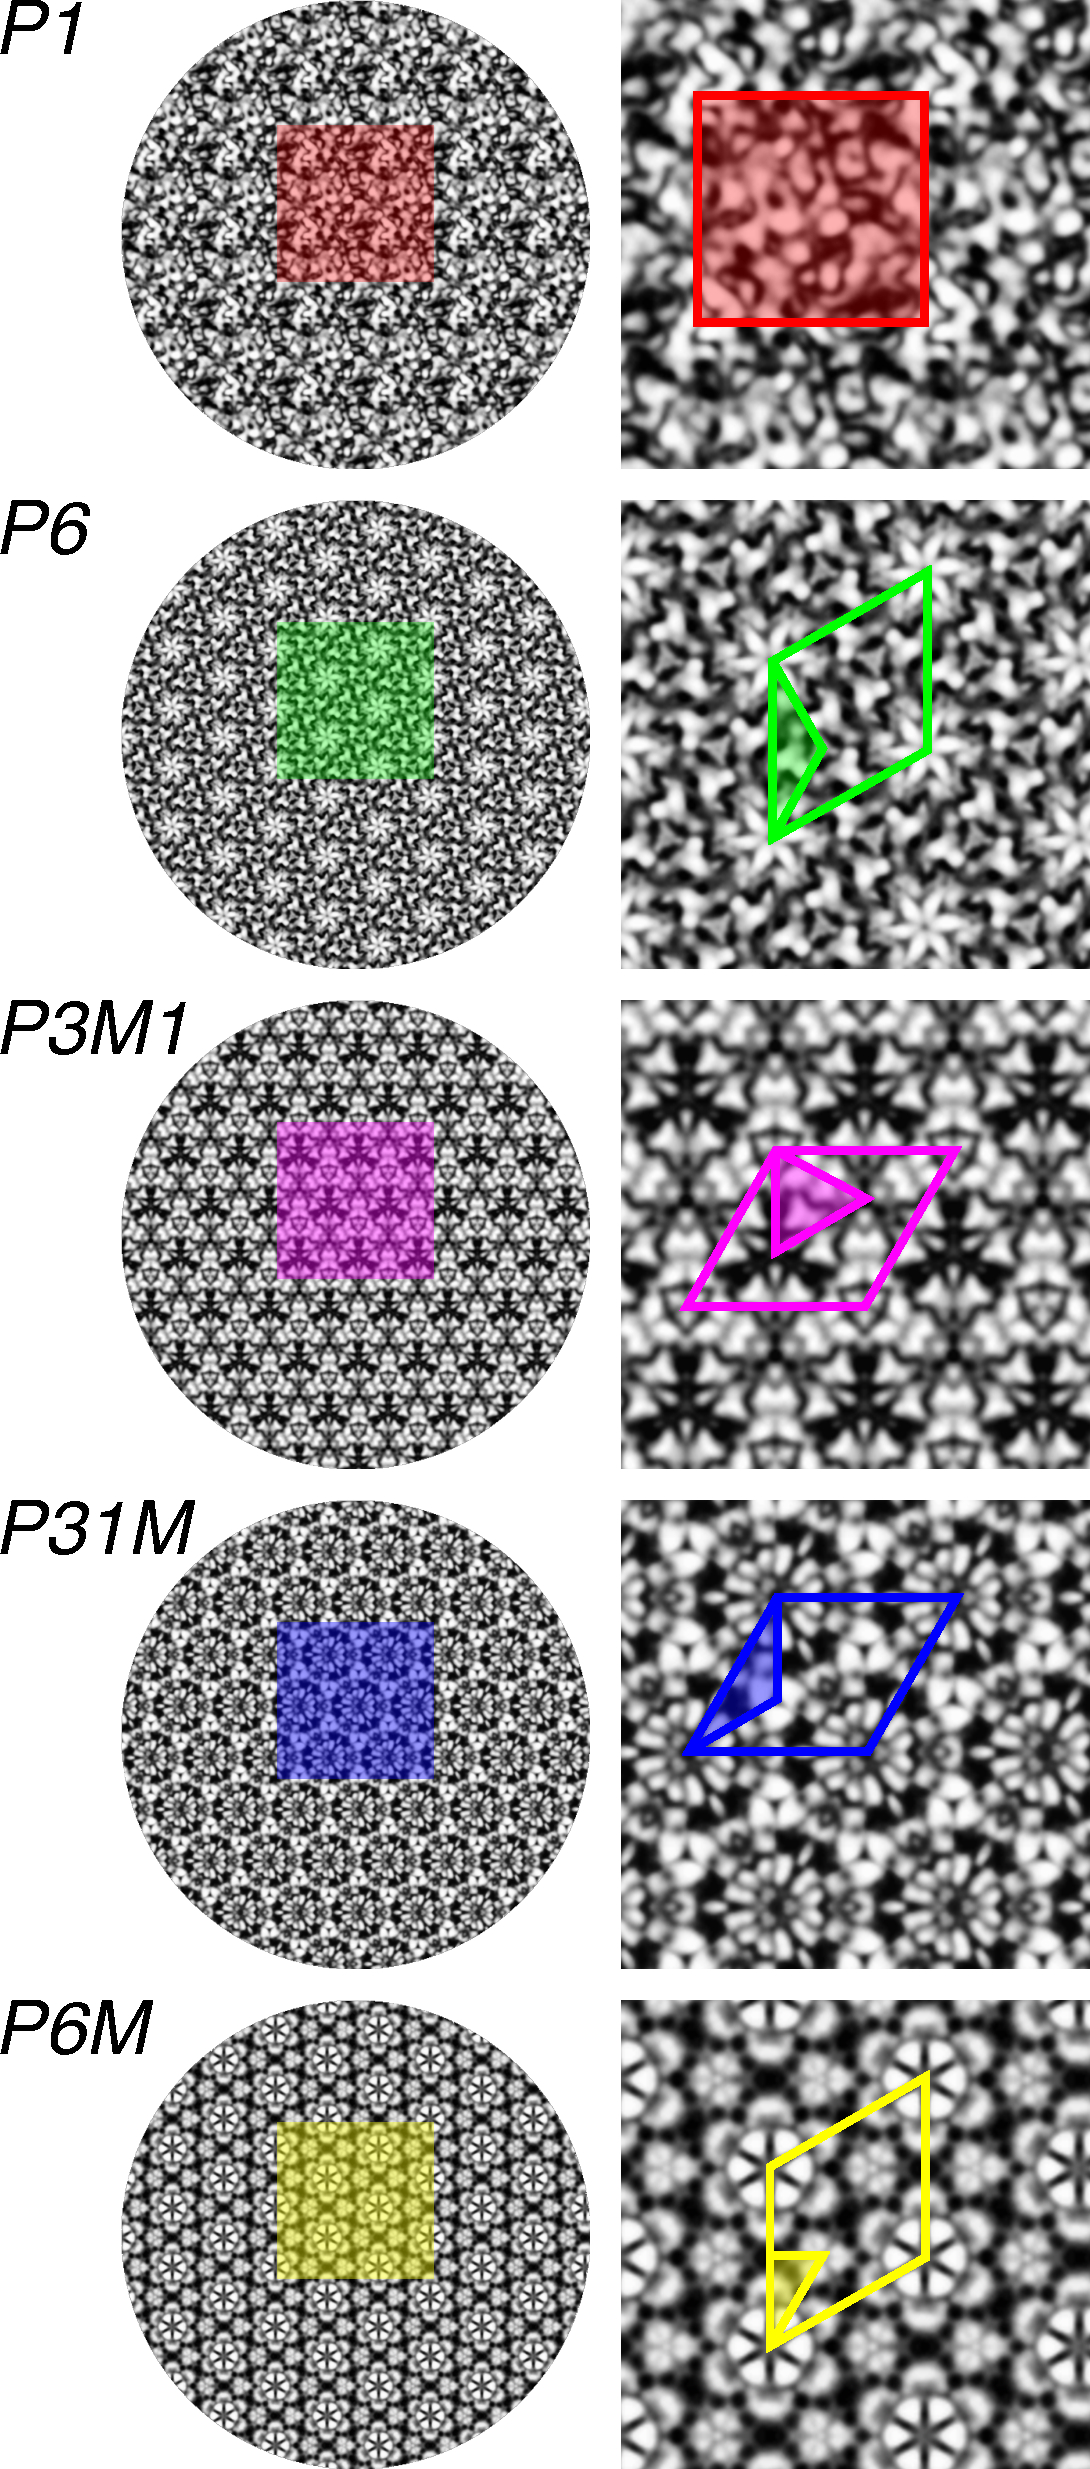
\includegraphics[width=0.44\textwidth]{./figures/wpg_structure.pdf}
>>>>>>> Stashed changes
	\caption{The fundamental region and lattice structure of the five wallpaper groups used in the study. The complete wallpaper is shown in the left-hand column with a shaded region that is repeated and enlarged in the right-hand column. The colored outline in the enlarged region indicates the repeating lattice for each group, while the shaded area indicates the fundamental region (see text). For \textit{P1} the fundamental region covers the entire lattice. Note that even though \textit{P6} and \textit{P31M} have the same fundamental region and lattice shapes, they differ in terms of the symmetries present within the lattice - most notably, \textit{P31M} contains reflection symmetry while \textit{P6} does not. The symmetry content of each group is detailed on the wallpaper group \href{https://en.wikipedia.org/wiki/Wallpaper_group}{wikipedia page}.}
	\label{fig:wpg_structure}
\end{wrapfigure}
Brain imaging studies using functional MRI \citep{RN1725} and EEG \citep{RN1959,kohler_clarke_2021} has shown that the human visual system carries detailed and precise representations of the symmetries within the individual wallpaper groups, and functional MRI evidence from macaque monkeys reveal similar representations in analogous areas of the macaque visual system \citep{audurier_symmetry_2021}.

These representations, complex as they are, do not appear to be readily available for driving conscious behaviour: Humans have limited intuitive sense of group membership for wallpaper group exemplars, as evidenced by behavioral experiments showing that although naïve observers can distinguish many of the wallpaper groups \citep{RN1253}, they tend to sort exemplars into fewer (4-12) sets than the number of wallpaper groups, often placing exemplars from different wallpaper groups in the same set \citep{RN172}. Wallpaper groups are nonetheless visually compelling and anecdotally we have observed that exemplars from a given group can be quite perceptually diverse. This observation inspired the current study, in which we use the behavioral sorting approach to probe the perceptual self-similarity of different exemplars from the same wallpaper group, and assess the extent to which self-similarity varies across five groups. 

<<<<<<< Updated upstream
We algorithmically generated 20 well-matched exemplars from each group (see Figures \ref{fig:wpg_structure} and \ref{fig:wpg_exemplars} for a selection of the exemplars, and the \nameref{methods} section for details on how they were generated) and printed them out on white cardstock. We then gave participants the 20 cards with exemplars from each wallpaper group, and asked them to freely sort them into as many subsets as they wished based on any criteria they saw appropriate. This approach allowed us to compare the five wallpaper groups, both in terms of how many subsets participants generated, and also in terms of \textit{jaccard index}, a summary statistic capturing the similarity across exemplar pairs for each group. Within each group, we were also able to identify exemplar pairs that were rated as highly similar and highly dissimilar. Our main conclusion is that \textit{P1} was systematically less self-similar than the any other groups, while the other four other groups could not be distinguished on these measures.
\begin{figure}[t]
=======
We algorithmically generated 20 well-matched exemplars from each group (see Figures \ref{fig:wpg_structure} and \ref{fig:wpg_exemplars} for a selection of the exemplars, and the \nameref{methods} section for details on how they were generated) and printed them out on white cardstock. We then gave participants the 20 cards with exemplars from each wallpaper group, and asked them to freely sort them into as many subsets as they wished based on any criteria they saw appropriate.

\begin{figure}[H]
>>>>>>> Stashed changes
	\centering
	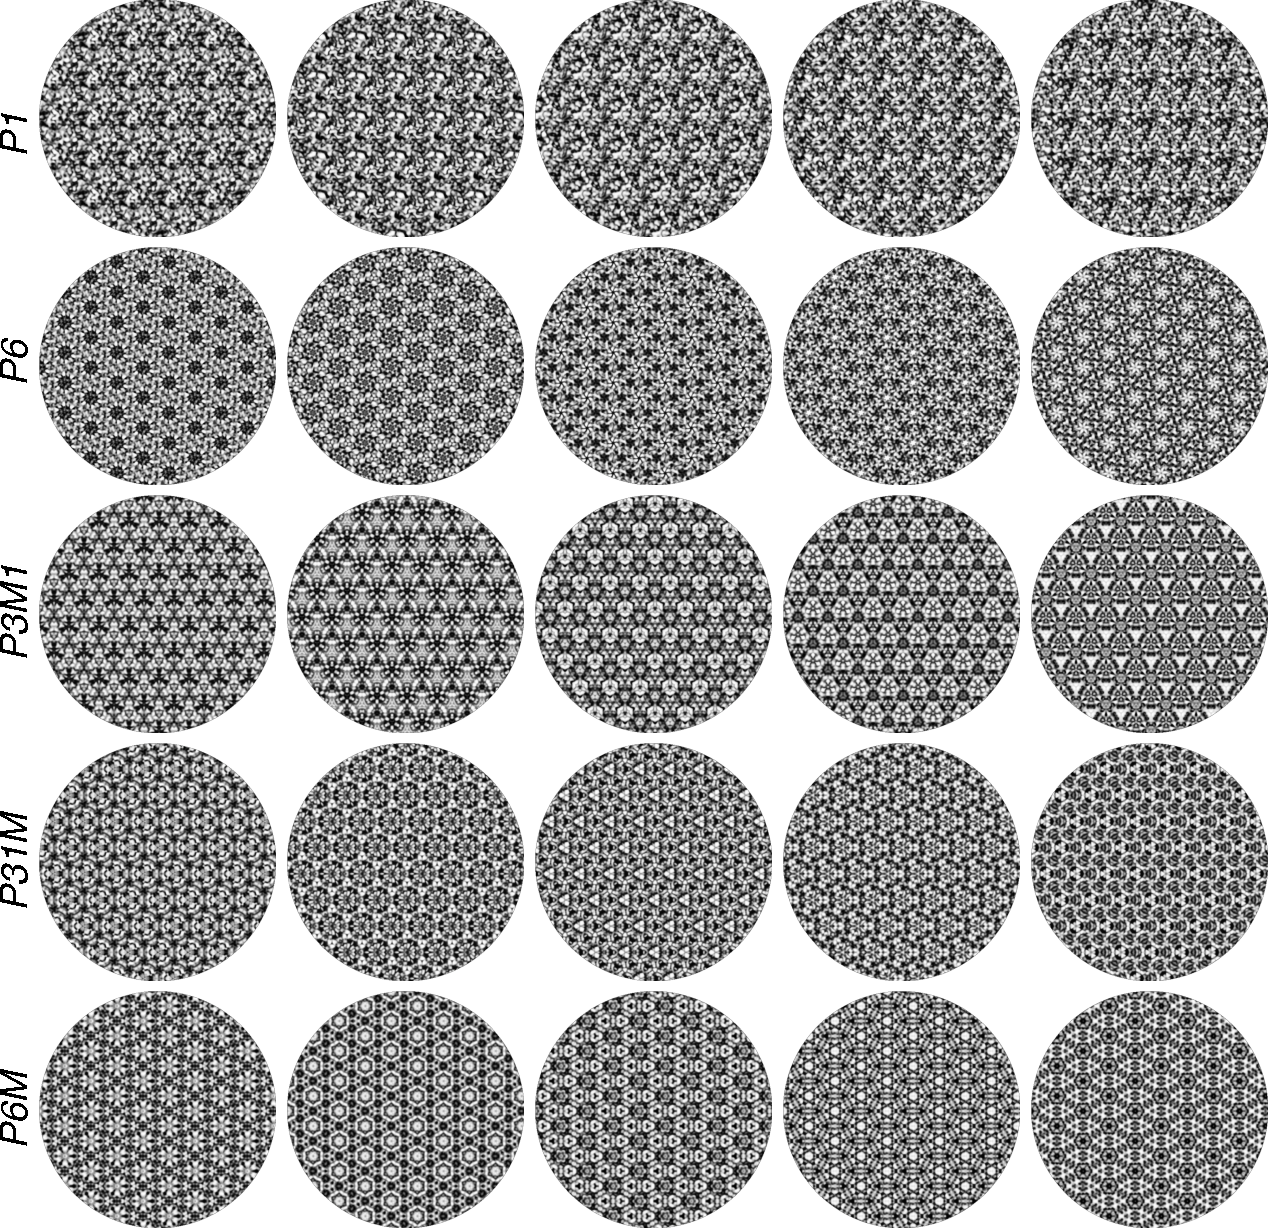
\includegraphics[width=\linewidth]{./figures//wpg_exemplars.pdf}
	\caption{5 of the 20 exemplars used for each group are shown to highlight the diversity among exemplars.}
	\label{fig:wpg_exemplars}
\end{figure}
<<<<<<< Updated upstream
=======




>>>>>>> Stashed changes

\section*{Results}
Wallpaper group \textit{P1} was less self-similar than the other four groups. This was evident in the number of sets generated for this group across participants, which was lower for \textit{P1} (median = 3) than for the other groups (median = 4-5, see Figure \ref{fig:n_sets_summary}). We confirmed this observation statistically by running a repeated measures analysis of variance (ANOVA) with group as the only factor, which revealed a significant effet of group ($F(4, 124) = 7.3301, p < 0.0001)$) \textcolor{red}{[SPHERICITY?!]}.
\begin{figure}[t]
	\centering
	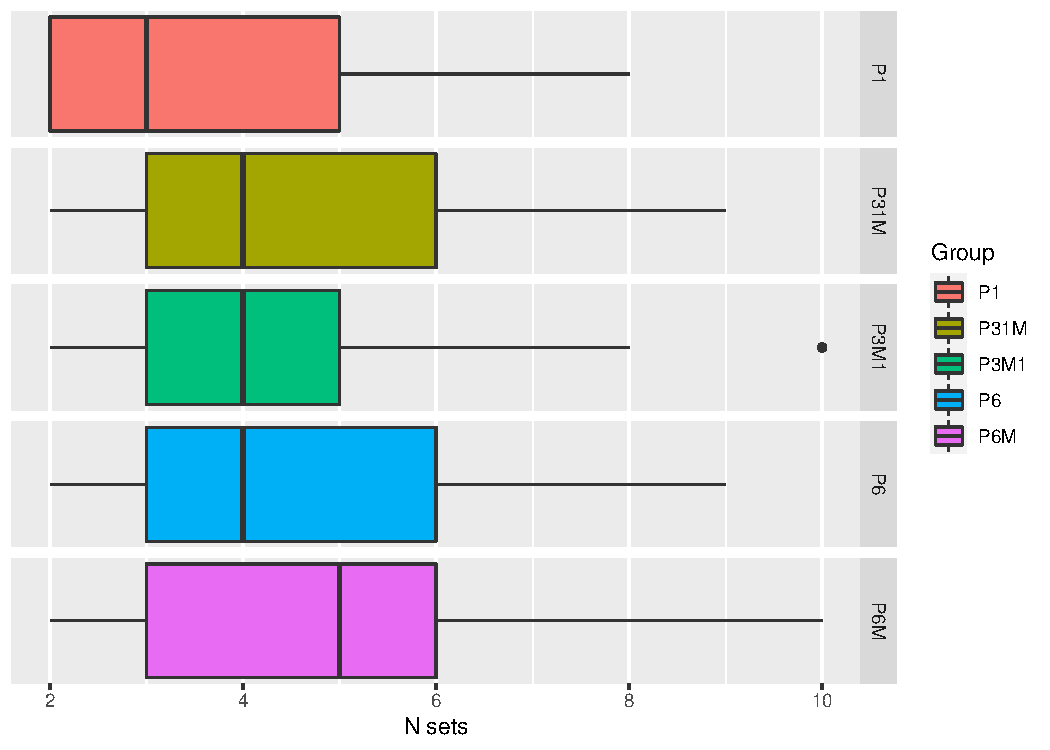
\includegraphics[width=\linewidth]{./figures/nsets_summary.pdf}
	\caption{Boxplots showing the number of subsets generated by participants for each of the wallpaper groups. The lower box boundary is the 25th percentile. The dark line in the box is the median. The upper box boundary is the 75th percentile. The “whiskers” show -/+ the interquartile range * 1.5.}
	\label{fig:n_sets_summary}
\end{figure}
Next, we computed the Jaccard index (see \nameref{methods}) across participants for every pairwise combination of exemplars in each group. This provides a measure of the similarity between exemplars for each group. \textit{P1} had sysmetically higher Jaccard Indices than the four other groups (see Figure \ref{fig:jaccard_summary}), as confirmed by a \textcolor{red}{XX}, which found significant effects of \textcolor{red}{XX}. The fact that the group (\textit{P1}) for which fewer subsets were generated also had higher Jaccard indices than the other groups illustrates the inherent link between the two measures: For wallpaper groups where the 20 exemplars are sorted into fewer subsets, each individual exemplar pair are more likely to be members of the same subset, and less likely to be members of distinct subsets, which in turn leads to higher Jaccard indices. These analysis thus allow us to conclude that out of the five groups tested, \textit{P1} is the only one that can be reliably differentiated based on our measures, being higher on self-similarity among the exemplars, and thus lower on diversity among exemplars. 

\begin{figure}[t]
	\centering
	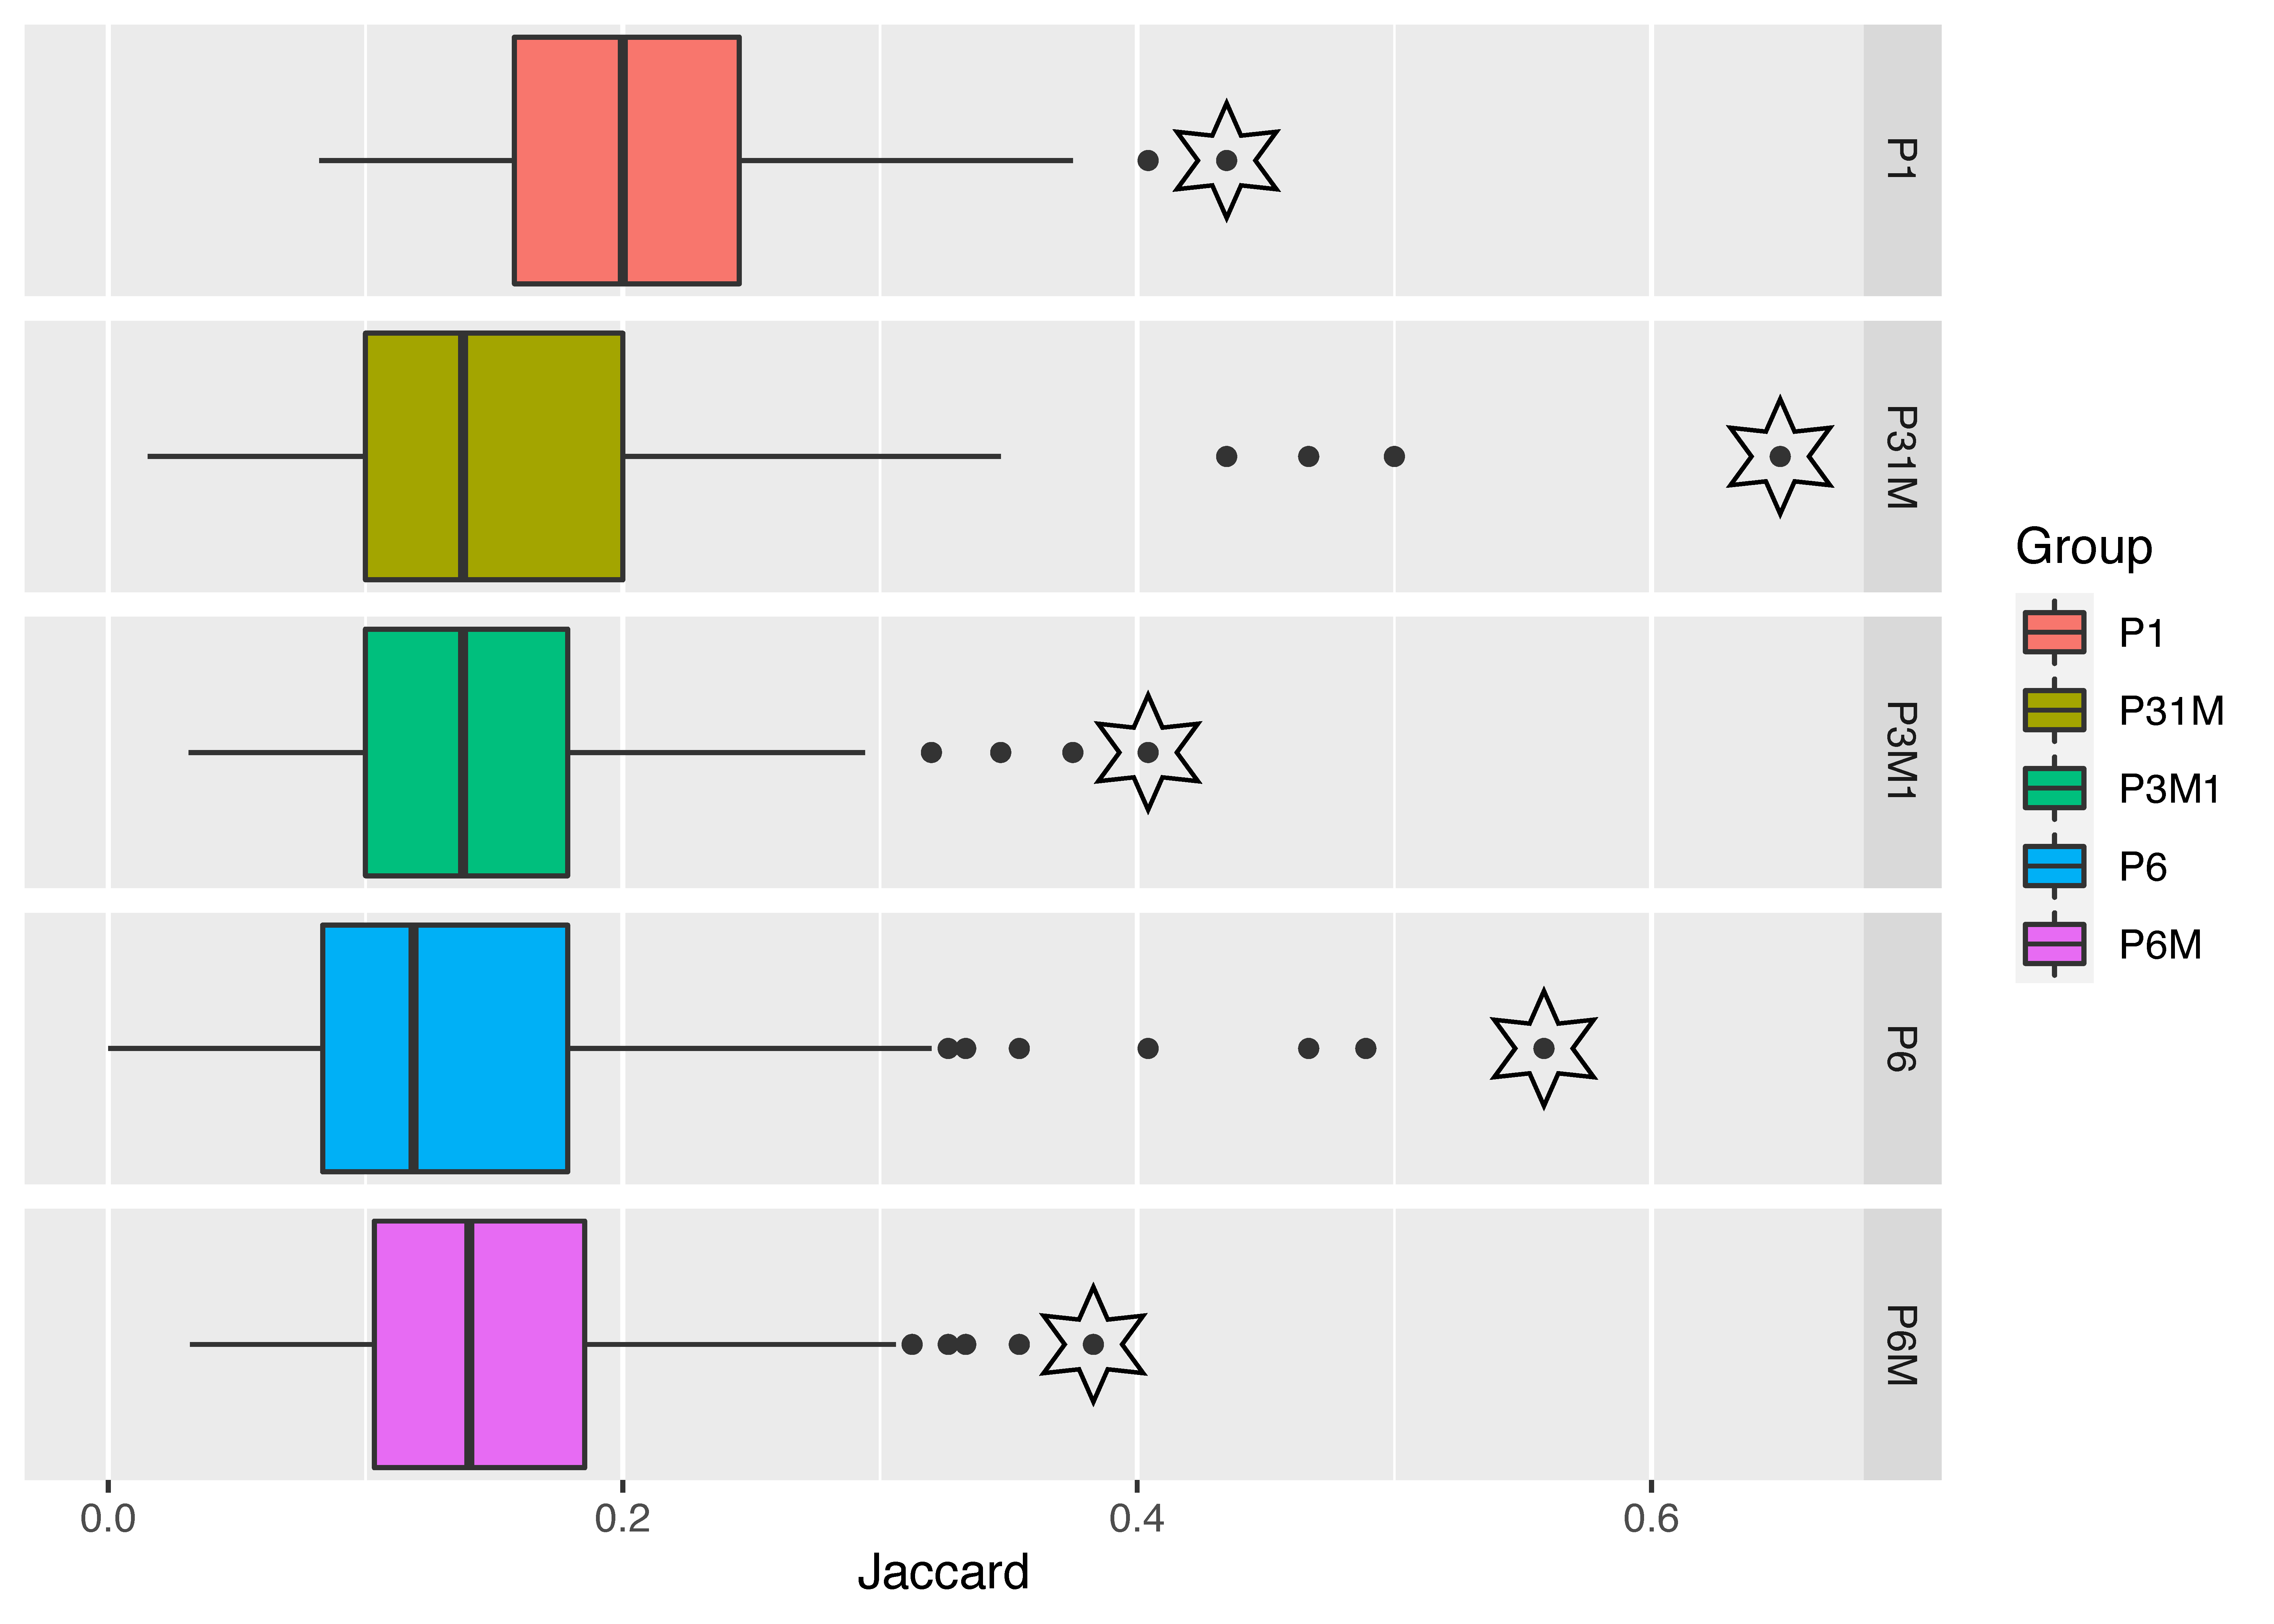
\includegraphics[width=\linewidth]{./figures/jaccard_summary.pdf}
	\caption{Boxplots showing Jaccard indices for every pairwise combination of exemplars in each of the wallpaper groups. Note that each data point here is the Jaccard index for a particular exemplar pair calculated across participants, unlike Figure \ref{fig:n_sets_summary} were each data point is a participant. The box boundary and whiskers follow the same logic as in Figure \ref{fig:n_sets_summary}. The exemplar pairs with the highest Jaccard indices have been highlighted with stars. Those outlier pairs are explored further in Figure \textcolor{red}{XX}}.
	\label{fig:jaccard_summary}
\end{figure}

The Jaccard indices also allow us to focus on exemplar pairs that have a high level of similarity relative to the rest of the pairs in the set. We do this by identifying outliers from each group, as identified with stars in \ref{fig:jaccard_summary}. For each exemplar in each outlier pair, we visualize the pairwise similarity (as measured by the Jaccard index) to every other exemplar in the set (see Figure \textcolor{red}{XX}). 

\section*{Discussion}

\section*{Materials and Methods}
\label{methods}

\begin{figure}[H]
	\centering
	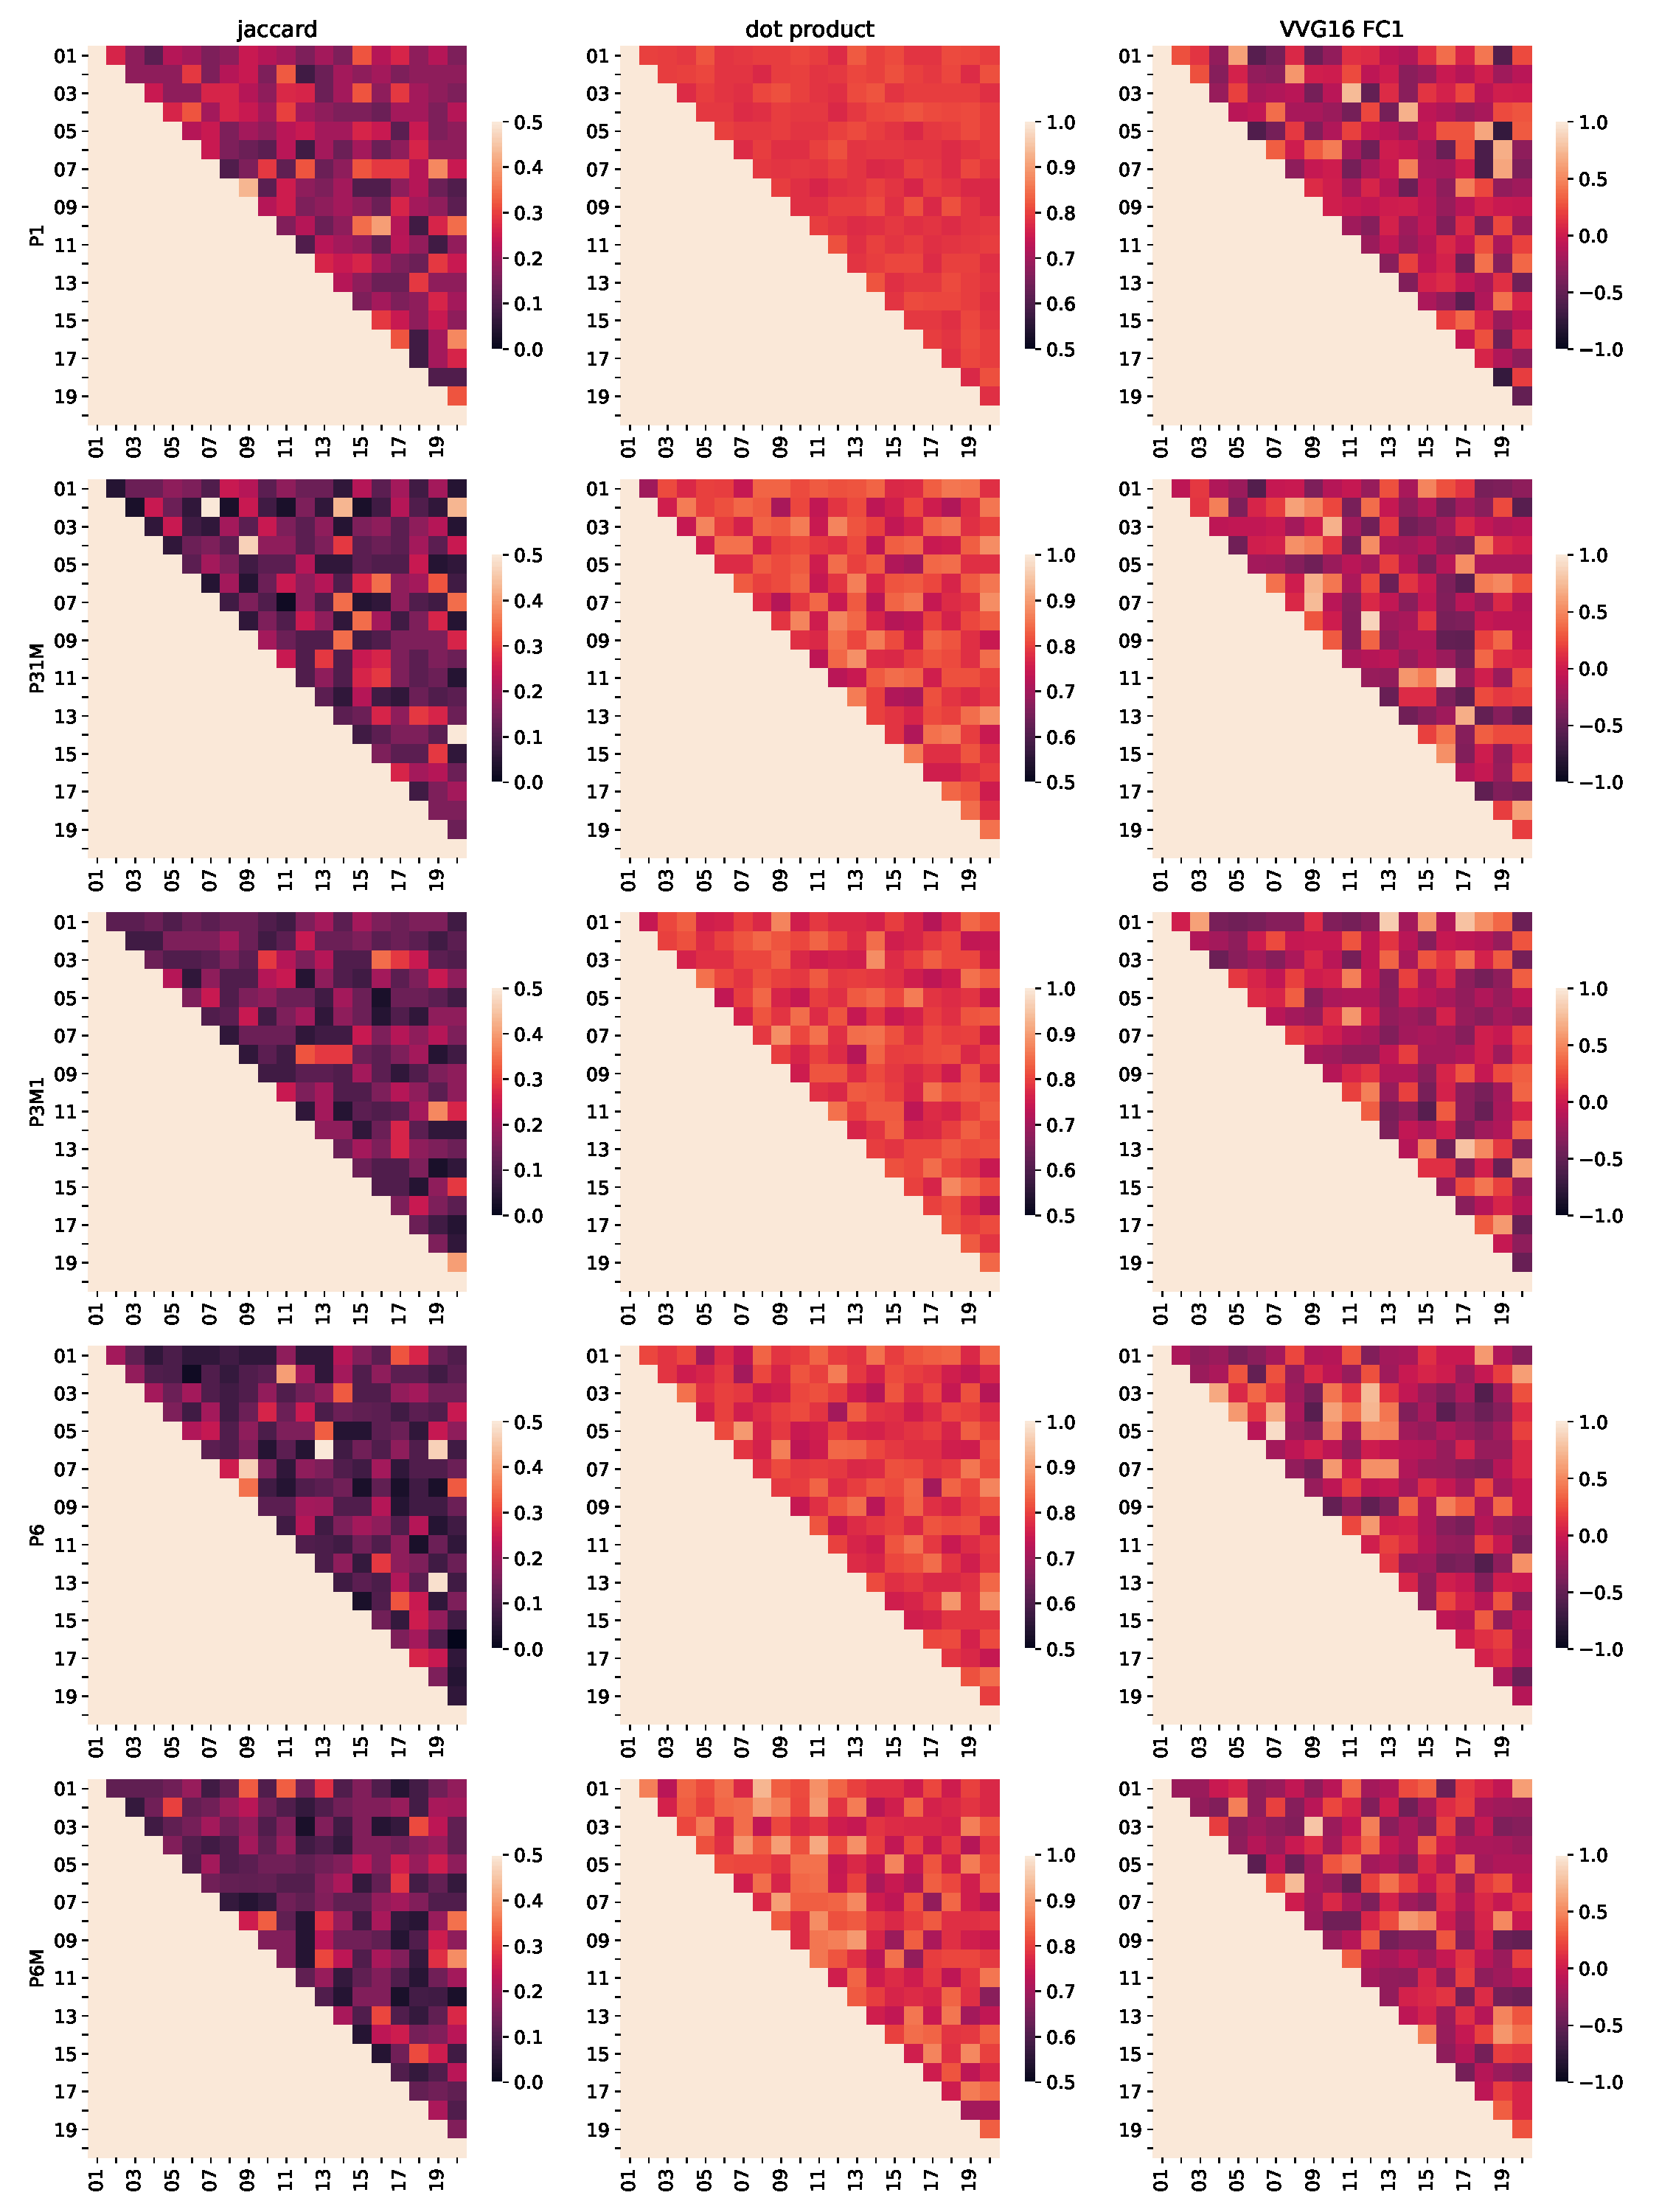
\includegraphics[width=\linewidth]{./figures/similarity_comparison.pdf}
	\caption{5 of the 20 exemplars used for each group are shown to highlight the diversity among exemplars.}
	\label{fig:similarity_comparison}
\end{figure}


\section*{Discussion}

\section*{Materials and Methods}
\label{methods}

\subsection*{Participants}
33 participants (9 Male, 24 Female), ranging in age between 18 and 35 completed this study. All participants had self reported 20/20 or corrected to 20/20 vision. We obtained written consent to participate from all participants under procedures approved by the Institutional Review Board of The Pennsylvania State University (\#38536). The research was conducted according to the principles expressed in the Declaration of Helsinki.

\subsection*{Stimulus Generation}
<<<<<<< Updated upstream
Five wallpaper groups (\textit{P1}, \textit{P3M1}, \textit{P31M}, \textit{P6} and \textit{P6M}) that has previously been shown to be high in self-similarity \citep{RN172}, were selected. 20 exemplars from each of these five wallpaper groups were generated using a modified version of the methodology developed by Clarke and colleagues\citep{RN172} that we have described in detail elsewhere\citep{RN1725}. Briefly, exemplar patterns for each group were generated from random-noise textures, which were then repeated and transformed to cover the plane, according to the symmetry axes and geometric lattice specific to each group. The use of noise textures as the starting point for stimulus generation allowed the creation of an almost infinite number of distinct exemplars of each wallpaper group. To make individual exemplars as similar as possible we replaced the power spectrum of each exemplar with the median across exemplars within a group. These images were printed onto white cardstock and cut into squares, allowing participants to manipulate the orientation of the images during the sorting tasks. Five exemplars from each group are shown (in reduced size) in \ref{fig:wpg_exemplars}. 

\subsection*{Procedure}
Participants were presented with the 20 exemplars of a single wallpaper group (i.e. P1, P3M1, P31M, P6, P6M) and instructed to sort them into subsets by placing them into piles. Participants were advised to sort the exemplars into as many piles as they deemed necessary based on whatever criteria they desired. There were no time constraints placed on this sorting task, and the participants were allowed to move exemplars between piles until they were satisfied with their classification. This method was then repeated for the remaining four wallpaper groups for each participant, with group presentation order randomized between participants. These tasks were carried out on a large table with sufficient space to randomly lay out all twenty exemplars of each set, illuminated by normal overhead room lighting. Upon completion of each sorting task, participants were asked to verbalize which features they used to sort the exemplars. After completion of all five sorting tasks, participants were asked which if they had a distinct method for sorting the images, and if any wallpaper group was particular easy or difficult to sort.

\subsection*{Generating the Jaccard Index}
The data was prepared for analysis by creating one binary variable for each subset created by each participant within a sorting task. Then, each exemplar was assigned a value of one (1) if it was included in a subset, or a value zero (0) if it was not. Next, the similarity of each pair of exemplars within a sorting task was calculated using the Jaccard index, a measure of similarity and diversity for binary data. This index is calculated by the equation  \[ J = \frac{x}{x + y + z} \] with x representing the number of subsets that contained both exemplars, and y and z the number of subsets that contain only one exemplar of the pair \citet{capra_factor_2005}, across participants. Thus, the Jaccard index is the ratio of the number of subsets containing both exemplars of a pair to the number of subsets containing at least one of the exemplars of a pair, thereby excluding subsets with joint absences.
=======
Five wallpaper groups (\textit{P1}, \textit{P3M1}, \textit{P31M}, \textit{P6} and \textit{P6M}) that has previously been shown to be high in self-similarity \citep{RN172}, were selected. 20 exemplars from each of these five wallpaper groups were created by tiling fundamental domains generated from random-dot white noise, resulting in a total of 100 distinct stimuli. These white noise fundamental domains had an area of ~4096 pixels, and were either square, rectangular, or triangular, depending on the symmetry group they represented. The advantages conferred by using white noise include the ability to generate numerous exemplars of the same wallpaper group and the absence of pattern discontinuities after tiling. These images were printed onto white cardstock and cut into squares, allowing participants to manipulate the orientation of the images during the sorting tasks. All stimuli are depicted (in reduced size) in Appendix A, organized by wallpaper group. 

Exemplars from the different wallpaper groups were generated using a modified version of the methodology developed by Clarke and colleagues\citep{RN172} that we have described in detail elsewhere\citep{RN1725}. Briefly, exemplar patterns for each group were generated from random-noise textures, which were then repeated and transformed to cover the plane, according to the symmetry axes and geometric lattice specific to each group. The use of noise textures as the starting point for stimulus generation allowed the creation of an almost infinite number of distinct exemplars of each wallpaper group. To make individual exemplars as similar as possible we replaced the power spectrum of each exemplar with the median across exemplars within a group. We then generated control exemplars that had the same power spectrum as the exemplar images by randomizing the phase of each exemplar image. The phase scrambling eliminates rotation, reflection and glide-reflection symmetries within each exemplar, but the phase-scrambled images inherent the spectral periodicity arising from the periodic tiling. This means that all control exemplars, regardless of which wallpaper group they are derived from, are transformed into another symmetry group, namely \textit{P1}. \textit{P1} is the simplest of the wallpaper groups and contains only translations of a region whose shape derives from the lattice. Because the different wallpaper groups have different lattices, \textit{P1} controls matched to different groups have different power spectra. Our experimental design takes these differences into account by comparing the neural responses evoked by each wallpaper group to responses evoked by the matched control exemplars.

\subsection*{Procedure}
Participants were presented with the 20 exemplars of a single wallpaper group (i.e. P1, P3M1, P31M, P6, P6M) and instructed to sort them into subsets by placing them into piles. Participants were advised to sort the exemplars into as many piles as they deemed necessary based on whatever criteria they desired. There were no time constraints placed on this sorting task, and the participants were allowed to move exemplars between piles until they were satisfied with their classification. This method was then repeated for the remaining four wallpaper groups for each participant, with group presentation order randomized between participants. These tasks were carried out on a large table with sufficient space to randomly lay out all twenty exemplars of each set, illuminated by normal overhead room lighting. 
Upon completion of each sorting task, participants were asked to verbalize which features they used to sort the exemplars. After completion of all five sorting tasks, participants were asked which if they had a distinct method for sorting the images, and if any wallpaper group was particular easy or difficult to sort.

\subsection*{Generating the Jaccard Index}
The data was prepared for analysis by creating one binary variable for each subset created by each participant within a sorting task. Then, each exemplar was assigned a value of one (1) if it was included in a subset, or a value zero (0) if it was not. Next, the similarity of each pair of exemplars within a sorting task was calculated using the Jaccard index, a distance similarity measure for binary data. This index is calculated by the equation  , with x representing the number of subsets that contained both 
exemplars, and y and z the number of subsets that contain only one exemplar of the pair (Capra, 2005). Thus, the Jaccard index is the ratio of the number of subsets containing both exemplars of a pair to the number of subsets containing at least one of the exemplars of a pair, thereby excluding subsets with joint absences.  

\subsection*{Comparing with DNNs and Dot Product}
>>>>>>> Stashed changes

% \begin{figure}[hptb]
%\centering
%\includegraphics[width=linewidth]{../figures/figure1.pdf}
%\caption{\textcolor{ForestGreen}{Subgroup relationships with indices 2 (solid lines) and 3 (dashed line) are shown in (A). All other relationships can be inferred by identifying the shortest path through the hierarchy, and multiplying the subgroup indices. For example, \textit{P1} is related to \textit{P6} through \textit{P6}\textrightarrow\textit{P3} (index 2) and \textit{P3}\textrightarrow\textit{P1} (index 3) so \textit{P1} is also a subgroup of \textit{P6} with index $3 \times 2 = 6$. We also show enlarged versions of some of the subgroup relationships involving \textit{P6} (B, shown in red) and \textit{PMM} (C, shown in blue) and highlight the symmetries within the subgroups to emphasize how the supergroup can be generated by adding additional transformations to the subgroup.}}
%\label{fig:subgroups}
%\end{figure}

% Bibliography
\begin{multicols}{2}
\small
\bibliographystyle{apalike} 
\bibliography{literature}
\end{multicols}

\end{document}